\subsection{Three-dimensional Linear Systems}
\label{ssec:three-dimensional-linear-systems}

Stepping up the game a little, we're taking a look at linear systems in three
variables. Just as a linear equations in two variables are lines in the real
plane, linear equations in three variables depict geometric objects called
`planes' in the three-dimensional real space, $\R^3$. They form the last class
of linear systems that can be efficiently visualized; with linear systems in
more variables being generally out of our perceptive reach.

Planes are the \emph{straight} objects in three-dimensional kind of sense. They
lock one direction of movement by making one variable wholly dependent on the
other two. An illustration is provided in \myref{figure}{fig:plane}.

\begin{figure}[ht]
 \centering
 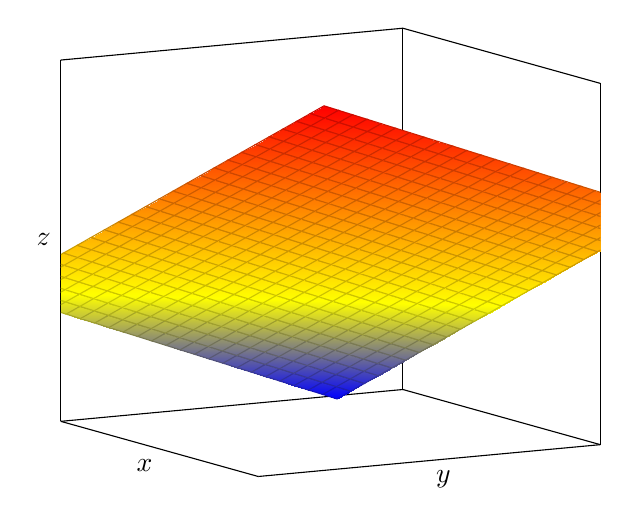
\begin{tikzpicture}
  \begin{axis}[
   view={60}{10},
   xlabel={$x$},
   ylabel={$y$},
   zlabel={$z$},
   zlabel style={rotate=90},
   xtick=\empty,
   ytick=\empty,
   ztick=\empty,
   xmin=-3,
   xmax=3,
   ymin=-5,
   ymax=5
  ]
   \addplot3[
    surf,
    colormap/hot,
    shader=faceted interp,
    ]({x}, {y}, {(2*x - y + 3) / 3});
  \end{axis}
 \end{tikzpicture}

 \caption{A \clb{plane} defined by the equation $2x - y - 3z = -3$.}
 \label{fig:plane}
\end{figure}

An \emph{underdetermined} system in three variables can contain either one or
two linear equations. In the former case, only one variable is dependent on the
other two -- we shall often call the independent variables by names such as
\emph{free variables} or \emph{parameters}. Both these names signify that a
substitution of any pair of real numbers in lieu of the two \emph{free
variables} yields a solution of the system.

For instance, the linear equation in \myref{figure}{fig:plane} is effectively a
linear system in three variables. We can choose any of the three variables to be
dependent and leave the other two free, giving thus three different descriptions
of \emph{the same} solution set. The following
equation~\eqref{eq:three-vars-one-eq} shows all of them with the chosen
dependent variable written on the left in typewriter font.
\begin{equation}
 \label{eq:three-vars-one-eq}
 \begin{array}{r l}
  \mathtt{x:} & \left\{ \left( \frac{y + 3z - 3}{2}, y, z \right) \mid y,z \in \R
  \right\}\\[1em]
  \mathtt{y:} & \left\{ \left( x, 2x - 3z + 3, z \right) \mid x,z \in \R
  \right\}\\[1em]
   \mathtt{z:} & \left\{ \left( x, y, \frac{2x - y + 3}{3} \right) \mid x,y \in
   \R \right\}
 \end{array}
\end{equation}

Linear systems in three variables and two equations are also underdetermined.
Geometrically, they correspond to arrangements of two planes in space. Those two
planes can either be parallel -- leading to the system having no solution -- or
not -- intersecting in a straight line describable as a set of triples with
exactly one free variable. In a case similar to two-dimensional linear systems,
putting the system in question into echelon form \emph{can} reveal (albeit not
always) its geometric nature.

Consider the system
\begin{equation}
 \label{eq:two-parallel-planes}
 \begin{array}{r c r c r c r}
  x & - & y & + & 2z & = & 2\\
  2x & - & 2y & + & 4z & = & 9
 \end{array}.
\end{equation}
Subtracting $\mathtt{II - 2 \cdot I}$ produces
\[
 \begin{array}{r c r c r c r}
  x & - & y & + & 2z & = & 2\\
    &   &   &   &  0 & = & 5
 \end{array},
\]
clearly a system with no solution. Subsequently, the two corresponding planes
are parallel to each other. See them depicted in
\myref{figure}{fig:two-parallel-planes}.

\begin{figure}[ht]
 \centering
 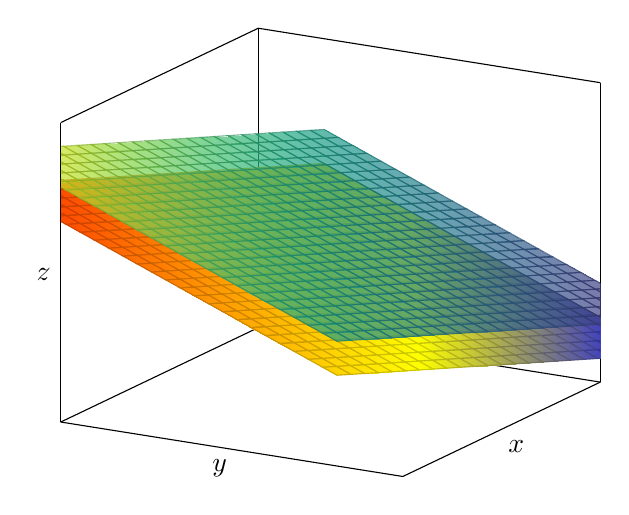
\begin{tikzpicture}
  \begin{axis}[
   view={-60}{20},
   xlabel={$x$},
   ylabel={$y$},
   zlabel={$z$},
   zlabel style={rotate=90},
   xtick=\empty,
   ytick=\empty,
   ztick=\empty,
   xmin=-3,
   xmax=3,
   ymin=-5,
   ymax=5
  ]
   \addplot3[
    surf,
    colormap/hot,
    shader=faceted interp,
   ]({x}, {y}, {(2 - x + y) / 2});
   \addplot3[
    surf,
    colormap/viridis,
    shader=faceted interp,
    opacity=0.7,
   ]({x}, {y}, {(9 - 2*x + 2*y) / 4});
  \end{axis}
 \end{tikzpicture}

 \caption{The two parallel planes from the
 system~\eqref{eq:two-parallel-planes}.}
 \label{fig:two-parallel-planes}
\end{figure}

A system of two non-parallel planes is presented below.
\begin{equation}
 \label{eq:two-non-parallel-planes}
 \begin{array}{r c r c r c r}
  x & - & y & + & 2z & = & 2\\
  2x & + & 3y & - & z & = & -1
 \end{array}
\end{equation}
By subtracting, once again, $\mathtt{II - 2 \cdot I}$, we put into the following
echelon form.
\[
 \begin{array}{r c r c r c r}
  x & - & y & + & 2z & = & 2\\
    &   & 5y & - & 5z & = & -5
 \end{array}
\]
The algorithm of Gauss-Jordan elimination limits our choice of parameters to the
ones left in the last row. We are hence to set either $y$ or $z$ loose while
caging the latter. Custom dictates to label as parameters all variables but the
first of the last row, making $z$ the victor. The rest is just
back-substitution. We calculate $y = z - 1$ and substitute into the first
equation to receive
\[
 x - (z - 1) + 2z = 2, \quad \text{hence} \quad x = 1 - z.
\]
It follows that \emph{one possible} description of the solution set of the
system~\eqref{eq:two-non-parallel-planes} is
\[
 \left\{ (1 - z, z - 1, z) \mid z \in \R\right\}.
\]
See it depicted in \myref{figure}{fig:two-non-parallel-planes}.
\begin{figure}[ht]
 \centering
 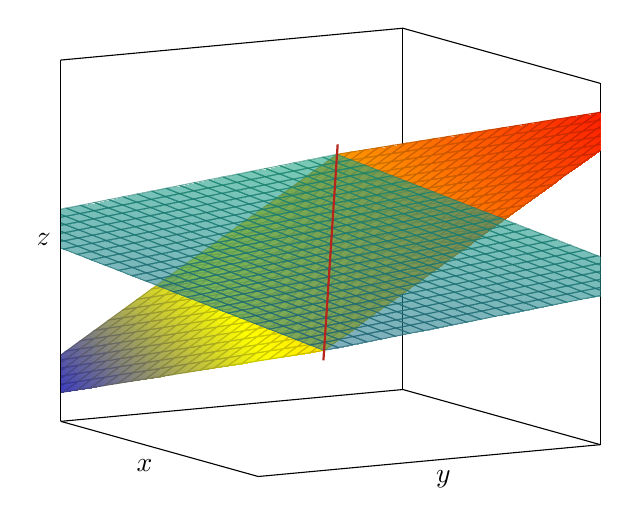
\begin{tikzpicture}
  \begin{axis}[
   view={60}{10},
   xlabel={$x$},
   ylabel={$y$},
   zlabel={$z$},
   zlabel style={rotate=90},
   xtick=\empty,
   ytick=\empty,
   ztick=\empty,
   xmin=-3,
   xmax=3,
   ymin=-5,
   ymax=5
  ]
   \addplot3[
    surf,
    colormap/hot,
    shader=faceted interp,
   ]({x}, {y}, {2*x + 3*y + 1});
   \addplot3[
    surf,
    colormap/viridis,
    shader=faceted interp,
    opacity=0.6
   ]({x}, {y}, {(2 - x + y) / 2});
  \addplot3[
   color=BrickRed,
   thick,
   smooth
  ]({x},{-x},{1-x});
  \end{axis}
 \end{tikzpicture}

 \caption{The two non-parallel planes from the
 system~\eqref{eq:two-non-parallel-planes} and their \clr{intersection}.}
 \label{fig:two-non-parallel-planes}
\end{figure}

Reaching the apex of `ideal' linear systems in three variables and three
equations, we stop to ponder the number of arrangements of three planes in
three-dimensional space. There are two obvious ones:
\begin{enumerate}
 \item All three planes are parallel to each other.
 \item Only two planes are parallel to each other.
\end{enumerate}
Corresponding to (1), resp. (2), is a linear system with two equations, resp.
one equation, with no solution.

As an example, consider the system
\begin{equation}
 \label{eq:two-parallel-one-not}
 \begin{array}{r c r c r c r}
  -x & + & 2y & - & z & = & 4\\
  x & - & 6y & + & z & = & 1\\
  x & - & 2y & + & z & = & 3
 \end{array}.
\end{equation}
Its echelon form looks like this:
\[
 \begin{array}{r c r c r c r}
  -x & + & 2y & - & z & = & 4\\
     & & -4y & & & = & 5\\
     & & & & 0 & = & 7
 \end{array}.
\]
Clearly, the third equation has no solution while the second does. This fact
alone, alas, carries not the full picture. To successfully determine that this
system corresponds to case (2) above, one need additionally take note of the
fact that the left side of row $\mathtt{III}$ of~\eqref{eq:two-parallel-one-not}
is a $(-1)$-multiple of row $\mathtt{I}$, meaning the two planes in question are
parallel.

The system~\eqref{eq:two-parallel-one-not} is shown in
\myref{figure}{fig:two-parallel-one-not}.
\begin{figure}[ht]
 \centering
 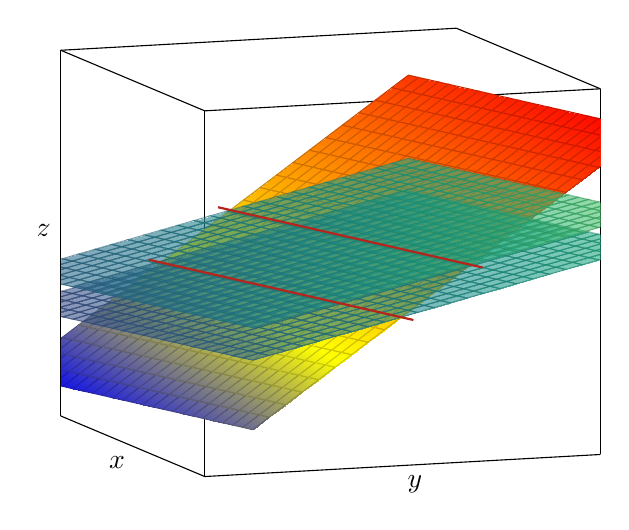
\begin{tikzpicture}
  \begin{axis}[
   view={110}{-10},
   xlabel={$x$},
   ylabel={$y$},
   zlabel={$z$},
   zlabel style={rotate=90},
   xtick=\empty,
   ytick=\empty,
   ztick=\empty,
   xmin=-3,
   xmax=3,
   ymin=-5,
   ymax=5
  ]
   \addplot3[
    surf,
    colormap/hot,
    shader=faceted interp
   ]({x}, {y}, {-x + 6*y + 1});
   \addplot3[
    surf,
    colormap/viridis,
    shader=faceted interp,
    opacity=0.6
   ]({x}, {y}, {-x + 2*y - 4});
   \addplot3[
    surf,
    colormap/viridis,
    shader=faceted interp,
    opacity=0.6
   ]({x}, {y}, {-x + 2*y + 3});
   \addplot3[
    color=BrickRed,
    thick,
    smooth
   ]({x},{1/2},{4-x});
   \addplot3[
    color=BrickRed,
    thick,
    smooth
   ]({x},{-5/4},{-x - 13/2});
  \end{axis}
 \end{tikzpicture}

 \caption{Depiction of the system~\eqref{eq:two-parallel-one-not}.}
 \label{fig:two-parallel-one-not}
\end{figure}

Finally, there are three other possible arrangements of three planes in space:
\begin{enumerate}
 \setcounter{enumi}{2}
 \item non-parallel planes that fail to have a common intersection (the
  so-often-called `tent' configuration);
 \item non-parallel planes that meet in a single point;
 \item non-parallel planes that meet in a single line.
\end{enumerate}
The echelon form of a linear system is not enough to distinguish case (2) from
case (3). For instance, the echelon form of the system
\begin{equation}
 \label{eq:tent}
 \begin{array}{r c r c r c r}
  x & + & 2y & - & z & = & -1\\
  2x & - & 3y & + & 2z & = & 4\\
  -x & + & 5y & - & 3z & = & 0
 \end{array}
\end{equation}
can easily be computed to be
\[
 \begin{array}{r c r c r c r}
  x & + & 2y & - & z & = & -1\\
    & & -7y & + & 4z & = & 6\\
    & & & & 0 & = & 5
 \end{array}.
\]
Notice the likeness to the echelon form of the previously studied
system~\eqref{eq:two-parallel-one-not}. One equation without solution, two
solvable. Its visual representation is to be found in
\begin{figure}[ht]
 \centering
 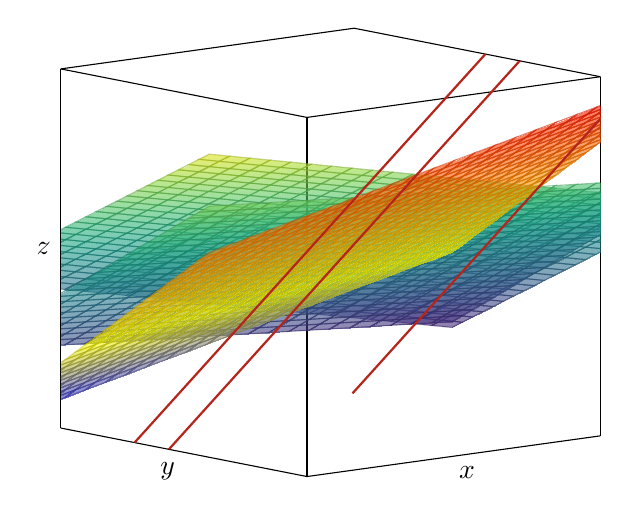
\begin{tikzpicture}
  \begin{axis}[
   view={40}{-10},
   xlabel={$x$},
   ylabel={$y$},
   zlabel={$z$},
   zlabel style={rotate=90},
   xtick=\empty,
   ytick=\empty,
   ztick=\empty,
   xmin=-3,
   xmax=3,
   ymin=-5,
   ymax=5
  ]
   \addplot3[
    surf,
    colormap/viridis,
    shader=faceted interp,
    opacity=0.6
   ]({x}, {y}, {(4 - 2*x + 3*y) / 2});
   \addplot3[
    surf,
    colormap/viridis,
    shader=faceted interp,
    opacity=0.6
   ]({x}, {y}, {(-x + 5*y) / 3});
   \addplot3[
    surf,
    colormap/hot,
    shader=faceted interp,
    opacity=0.6
   ]({x}, {y}, {x + 2*y + 1});
   \addplot3[
    color=BrickRed,
    thick,
    smooth
   ]({x},{2-4*x},{-7*x+5});
   \addplot3[
    color=BrickRed,
    thick,
    smooth
   ]({x},{-4*x - 3},{-7*x - 5});
   \addplot3[
    color=BrickRed,
    thick,
    smooth
   ]({x},{-4*x + 12},{-7*x + 20});
  \end{axis}
 \end{tikzpicture}

 \caption{Example of the `tent' arrangement of planes in~\eqref{eq:tent}.}
 \label{fig:tent-configuration}
\end{figure}

Without delving into visualisations of linear systems in three variables and
more than three equations -- which do not actually bring anything new to the
table -- we conclude the section with a few exercises.

\begin{exercise}{}{}
 Draw the following linear systems.
 \[
  \begin{array}{r c r c r}
   2x & + & y & = & 1\\
   3x & + & 2y & = & 3
  \end{array}
  \hspace{3em}
  \begin{array}{r c r c r}
   -x & + & y & = & 2\\
   2x & - & 2y & = & 5
  \end{array}
  \hspace{3em}
  \begin{array}{r c r c r}
   -x & - & y & = & 1\\
   3x & + & 2y & = & 0
  \end{array}
 \]
\end{exercise}

\begin{exercise}{}{}
 Without depicting them visually, determine the arrangement of planes
 corresponding to the linear system below.
 \[
  \begin{array}{r c r c r c r}
   2x & - & y & + & z & = & 3\\
   x & - & 3y & + & 4z & = & 1\\
   x & + & 2y & - & 3z & = & 2
  \end{array}
 \]
\end{exercise}

\begin{exercise}{}{}
 Find linear systems in three variables and three equations corresponding to
 cases (1), (4) and (5) in the text above.
\end{exercise}
